
\documentclass[12pt]{article}

% margin left and right with \setlength{\itemindent}{-.5in} %
\usepackage{enumitem}

% leave out section numbers in subsection numbering %
\usepackage[T1]{fontenc}
\renewcommand*\thesubsection{\arabic{subsection}}


% include Roman numerals for sections %
\renewcommand{\thesection}{\Roman{section}}
%Roman numerals for subsections like this \renewcommand{\thesubsection}{\Roman{subsection}}%
% include the package of the color%
\usepackage[usenames, dvipsnames]{color}
\usepackage[english]{babel}
\usepackage[utf8x]{inputenc}
\usepackage{amsmath}
\usepackage{graphicx}
\usepackage{subfiles}

%define your own color %
\definecolor{mygray}{gray}{0.9}
\begin{document}
	\listoffigures
	\title{Chapter 2 : Analysis and specification of requirements}
	\maketitle
	
	\section{Introduction}
	Being the first in the development cycle of the project, this phase is the most
	important. Indeed, it is during this period that the needs of the user are identified and specified. These requirements also represent the functionalities that should be present in the application, which also makes it possible to validate the application as the development progresses.
	\section{Actors Identification}
	\textbf{MassTer Insight web Application }was mainly designed to be used by \textbf{Data Analysts }in MMM agencies, which is the case of \textbf{MASS Analytics}, \textbf{Media Agencies }that have a MMM division, and \textbf{Advertisers }who have an in-house MMM team.
	
	\clearpage
	\newpage
	
	
	\section{Requirement Analysis}

	\subsection{Functional Requirements}
     
	These functional requirements express the expectations of different users for the product to be produced.
	\\
	\\
	In this part, we present the different functionalities and services that the application must ensure.
	
	CONNECT TO SERVER
	\begin{itemize}
		\setlength{\itemindent}{+.5in}
		\item \textbf{Connect To MassTer Server : } 
	\end{itemize}
	
	LOAD PROJECT
	\begin{itemize}
		\setlength{\itemindent}{+.5in}
     	\item \textbf{Load MassTer Insight Project : } 
    \end{itemize}	
 
 	MANAGE REPORT
 		\begin{itemize}
 			\setlength{\itemindent}{+.5in}
 			\item \textbf{Available Reports : } 
 			\item \textbf{Save a Report : }
 			\item \textbf{Remove a Report : }
 			\item \textbf{Load a Report : } 
 			\item \textbf{Available Channel : } 
 			\item \textbf{Seasonality Index Per Month : }
 			\item \textbf{Ignore Preset Laydown : }
 			\item \textbf{Budget Tolerance : }
 			\item \textbf{Revenue Tolerance : }
 			\item \textbf{Max Iteration  : }
 			\item \textbf{Max Iteration  : }
 			\item \textbf{Budget Range : }
 			\item \textbf{Total Budget : }
 			\item \textbf{Min Target : }
 			\item \textbf{Select Channel : }
 			\item \textbf{Max budget/Min Target/Set Budget per Channel : }
 	\end{itemize}
 
  	UPDATE
    \begin{itemize}
    	\setlength{\itemindent}{+.5in}
    	\item \textbf{Update a Report : }
   \end{itemize}

  	RUN
   \begin{itemize}
   	   \setlength{\itemindent}{+.5in}
 	   \item \textbf{Run new scenario : }
   \end{itemize}

    \clearpage
    \newpage

	\subsection{Non-Functional Requirements}
	\begin{itemize}
		\item \textbf{Ergonomics : }The application offers a user-friendly and easy-to-use interface without refer to particular knowledge.
		\item \textbf{Security : }
		\item \textbf{Modularity : }a code that is easy to maintain and simple to understand in order to ensure the scalability of application. 
	\end{itemize}
	\clearpage
	\newpage
	
	\section{Use Case Diagrams}
	\subsection{Global Use Case Diagram}
	\clearpage
	\newpage
	\begin{figure}[h]
		\centering
		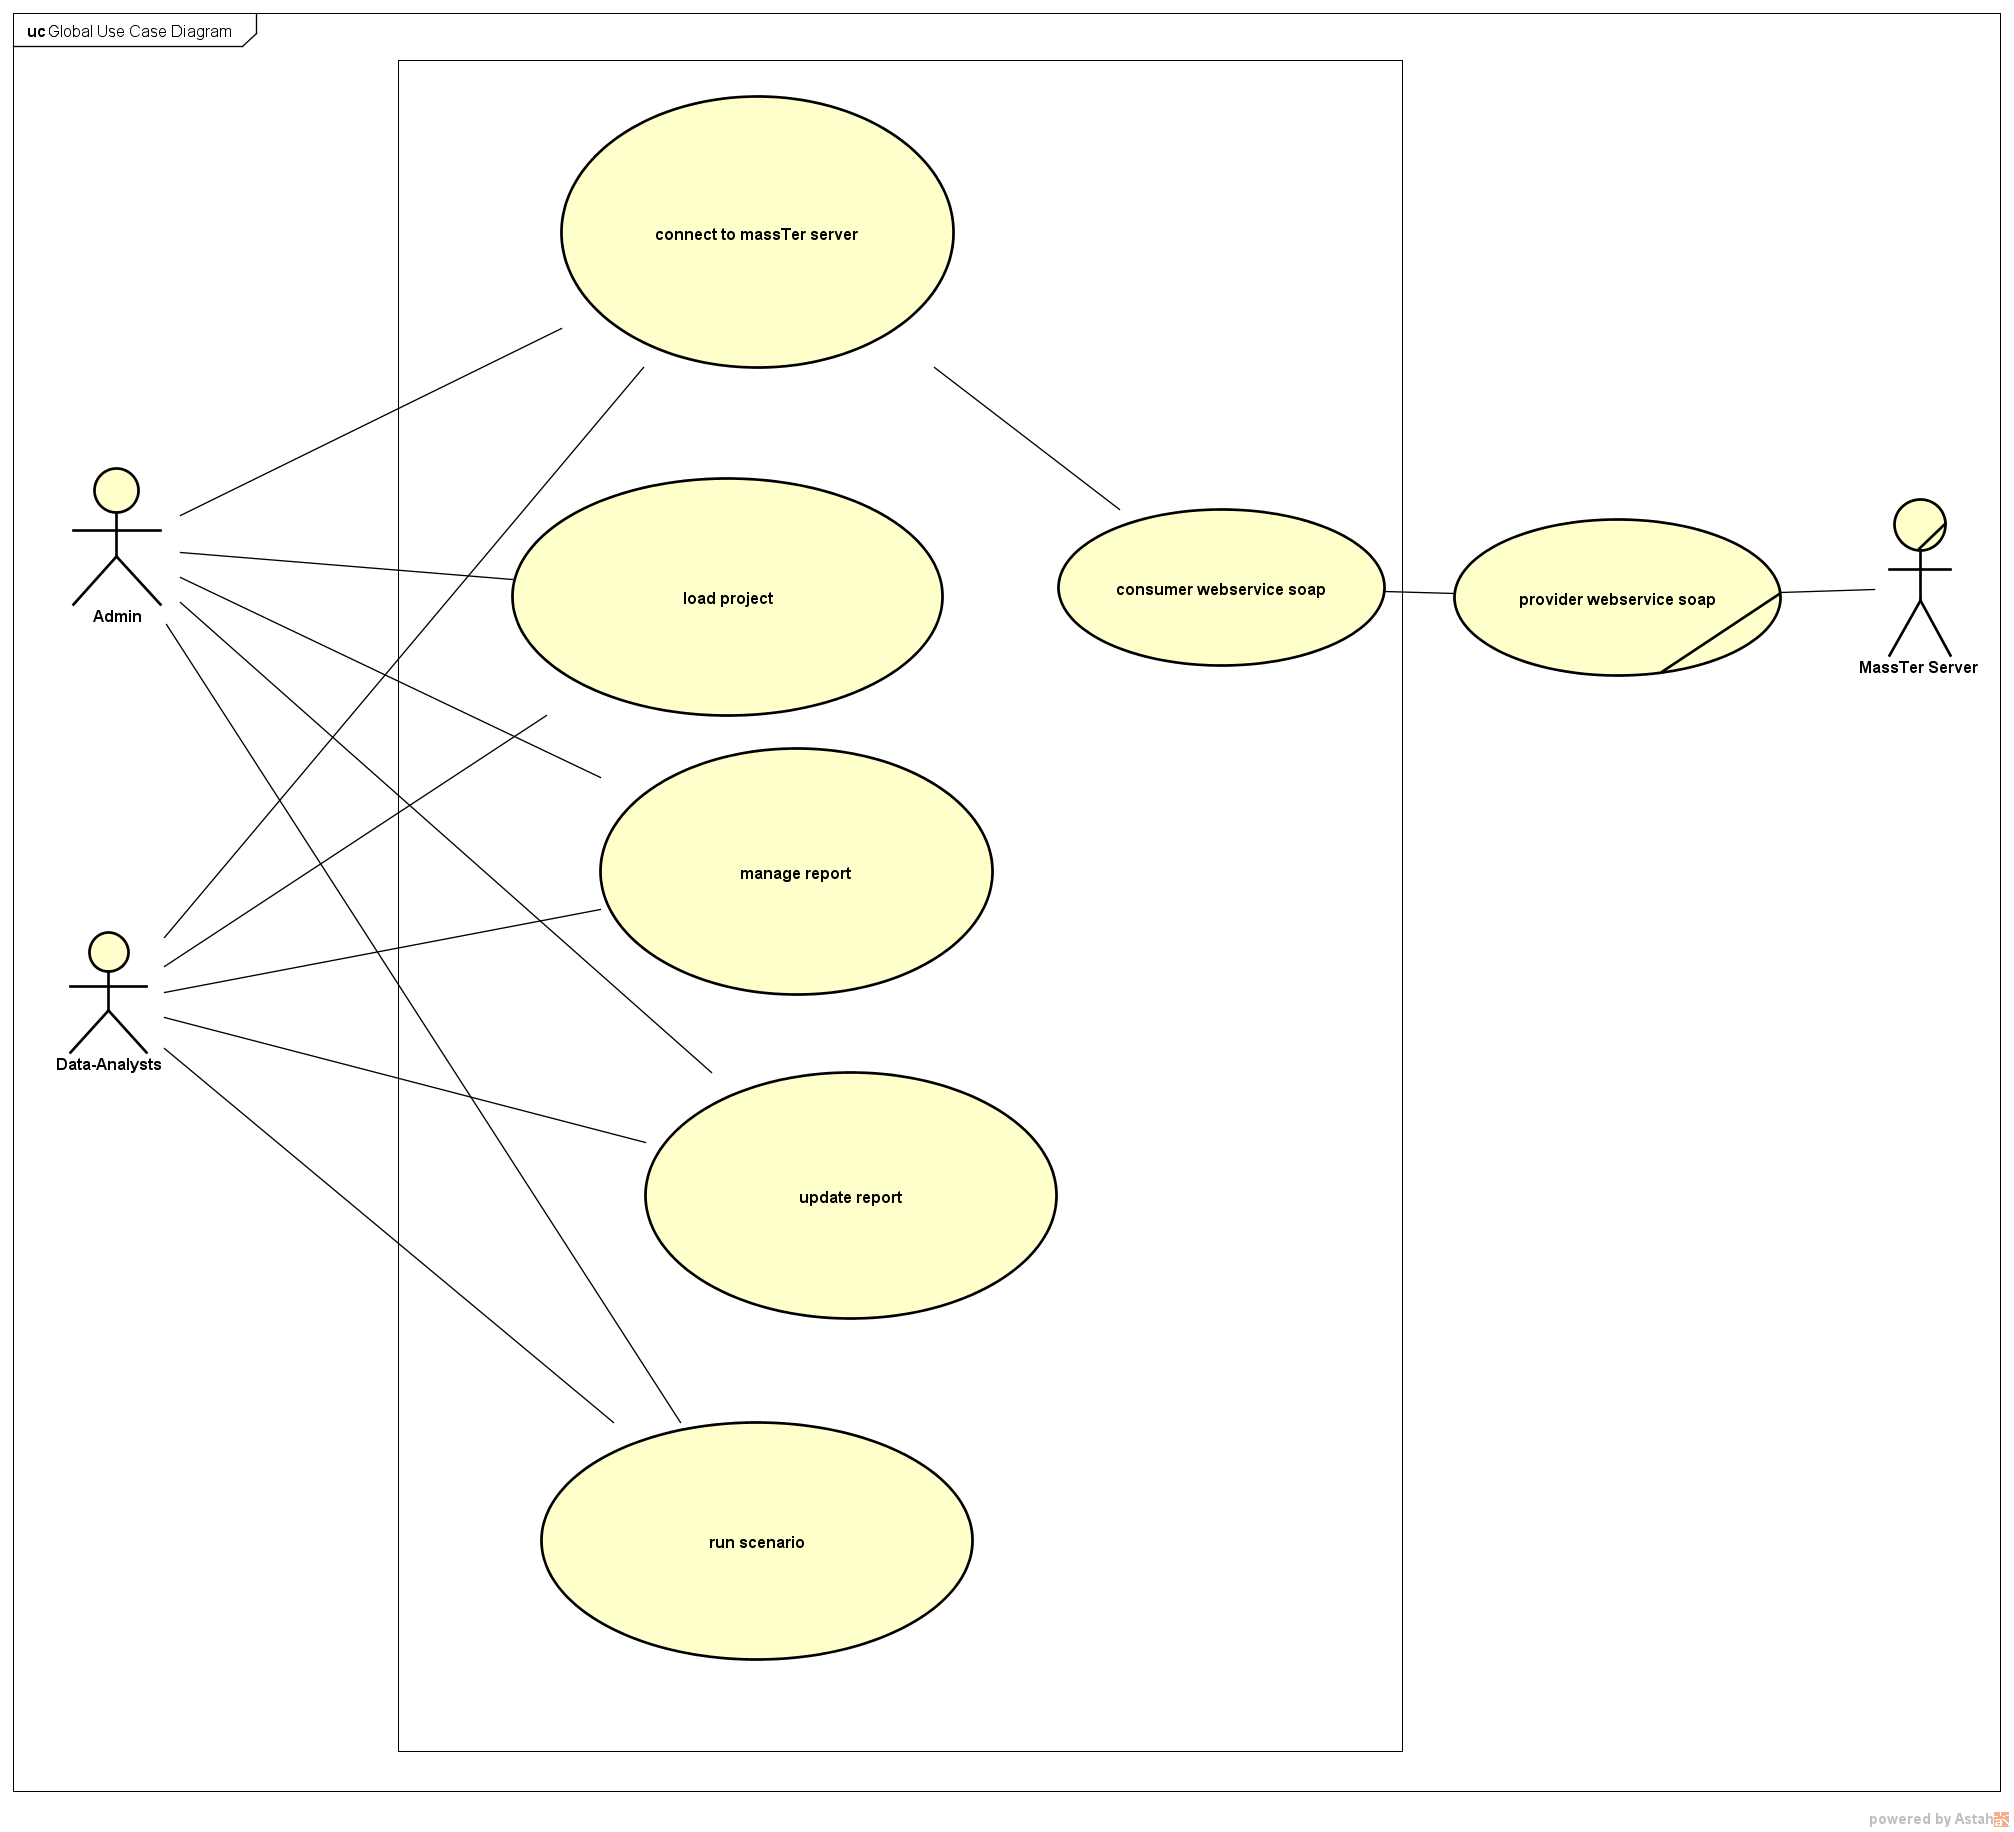
\includegraphics[width=1.0\textwidth]{GlobalUseCaseDiagram.png}
		\caption{Global Use Case Diagram}
		
	\end{figure}

\clearpage
\newpage


	\subsection{Detailed Use Case Diagrams}
	\clearpage
	\newpage
	 \subsubsection{connect to MassTer Server}
	 	\begin{figure}[h]
	 	\centering
	 	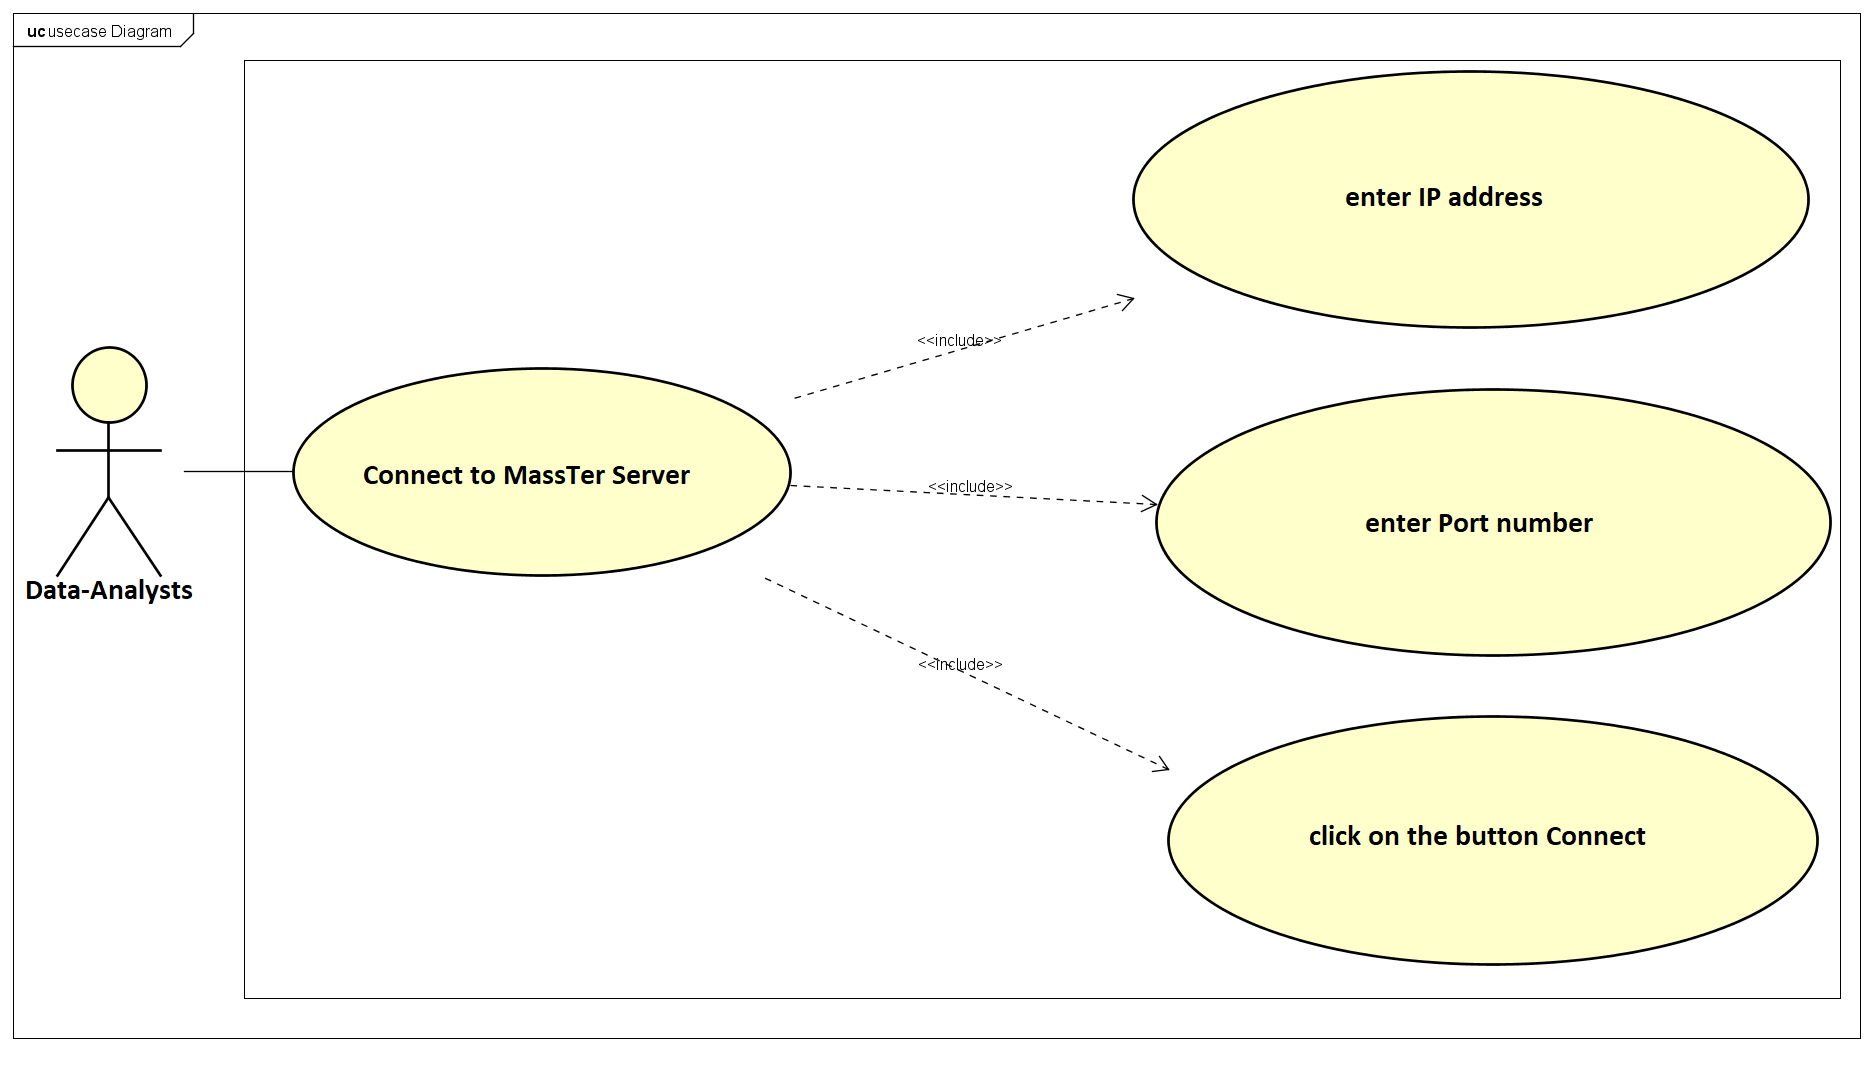
\includegraphics[width=1.0\textwidth]{connectToMassTerServer.png}
	 	\caption{connect to MassTer Server Use Case Diagram}
	 	
	 \end{figure}

  \newpage
 
 Description of the scenario ``connect to MassTer Server'' in the table below. 
 \\
 
 \begin{table}
 	\centering
 	\begin{tabular}{|c|p{10cm}|}
 		\hline 	
 		\textbf{Pre-conditions } & MassTer Server is running  \\ 
 		\hline                     
 		\textbf{Nominal Scenario } & \begin{enumerate}
 			\item The user click on the item MassTer Server in Main Menu.
 			\item The Application display a drop down. 
 			\item The user type MassTer Server IP address.
 			\item The user type MassTer Server port number.
 			\item The  user click on button connect. 
 		\end{enumerate} \\ 
 		\hline 
 		\textbf{Post-conditions} & The Application gets connected to MassTer Server. \\
 		\hline 
 	\end{tabular}
 \end{table}


 \clearpage
 \newpage
	 \subsubsection{consume web Service soap}
	 	 	\begin{figure}[h]
	 	\centering
	 	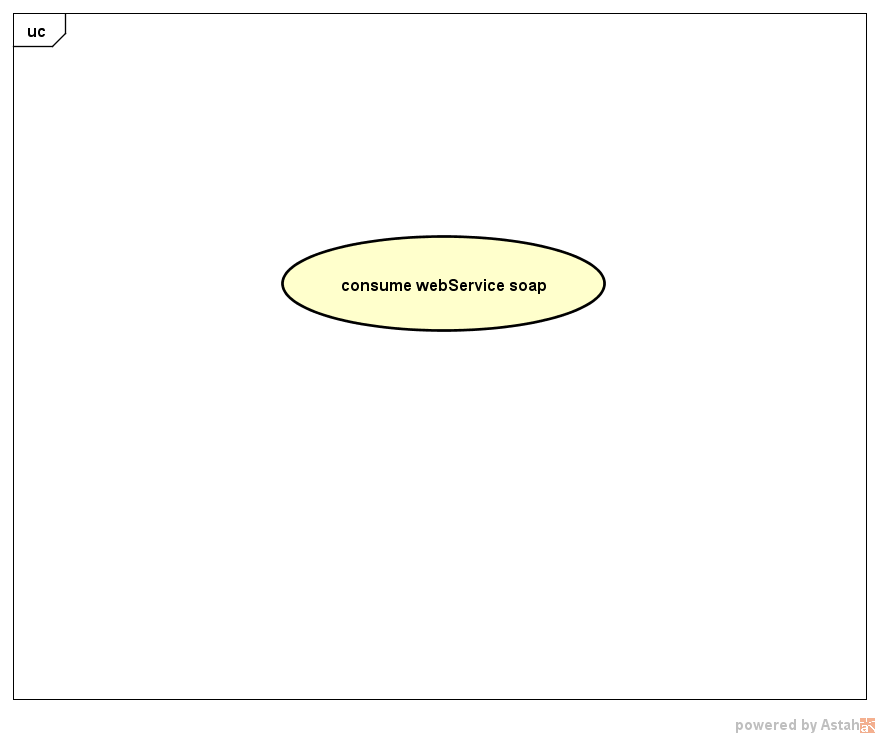
\includegraphics[width=1.0\textwidth]{consumewebServicesoap.png}
	 	\caption{consume web Service soap Use Case Diagram}
	 	
	 \end{figure}
 Description of the scenario ``consume web Service soap'' in the table below.
  \begin{table}
 	\centering
 	\begin{tabular}{|c|p{10cm}|}
 		\hline 	
 		\textbf{Pre-conditions } & MassTer Server is running  \\ 
 		\hline                     
 		\textbf{Nominal Scenario } & \\ 
 		\hline 
 		\textbf{Post-conditions} & ... \\
 		\hline 
 	\end{tabular}
 \end{table}
 \clearpage
 \newpage

	 \subsubsection{provide web Service soap} 
	 	\begin{figure}[h]
	 	\centering
	 	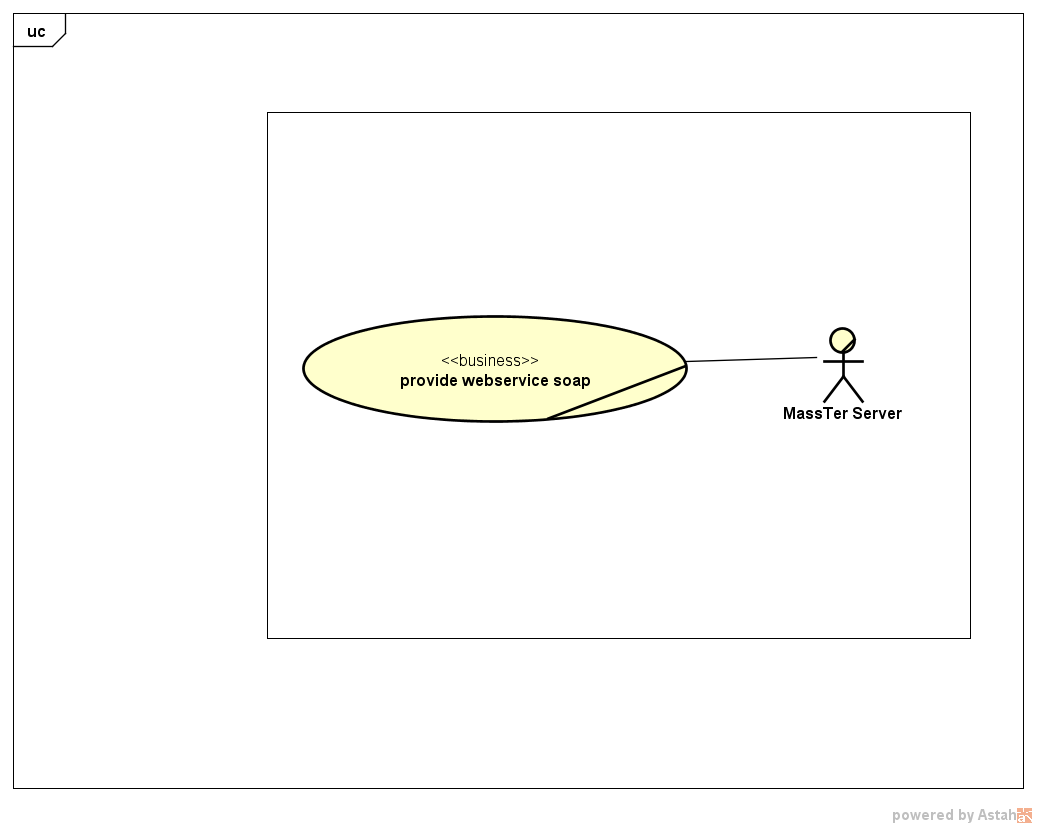
\includegraphics[width=1.0\textwidth]{provideWebServiceSoap.png}
	 	\caption{provide web Service soap Use Case Diagram}
	 	
	 \end{figure}
  Description of the scenario ``consume web Service soap'' in the table below.
   \begin{table}
  	\centering
  	\begin{tabular}{|c|p{10cm}|}
  		\hline 	
  		\textbf{Pre-conditions } & MassTer Server is running  \\ 
  		\hline                     
  		\textbf{Nominal Scenario } & \\ 
  		\hline 
  		\textbf{Post-conditions} & ... \\
  		\hline 
  	\end{tabular}
  \end{table}
 \clearpage
 \newpage
	 \subsubsection{load project}
	 	\begin{figure}[h]
	\centering
	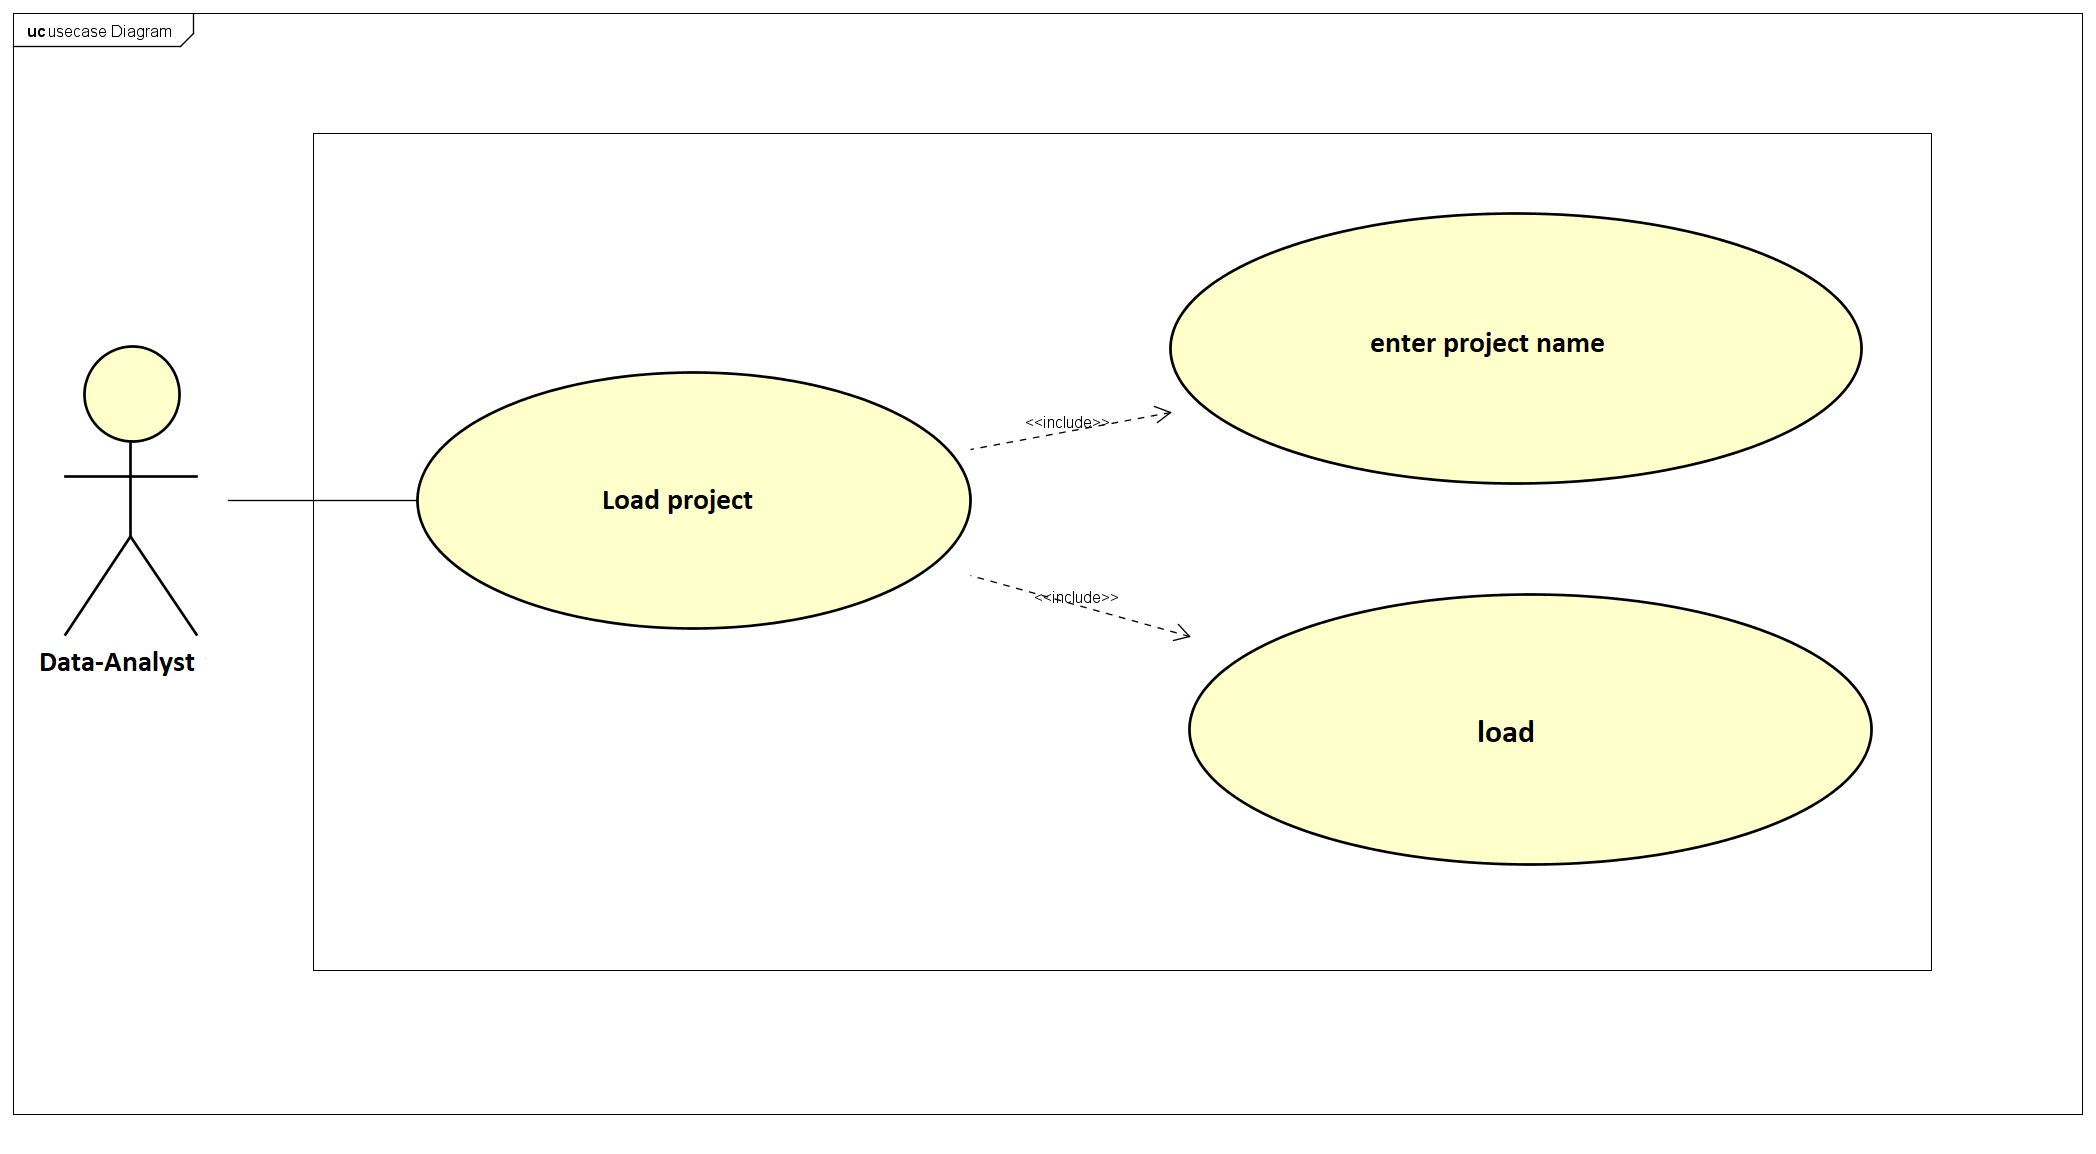
\includegraphics[width=1.0\textwidth]{loadProject.png}
	\caption{load project Use Case Diagram}
	
	\end{figure}

 Description of the scenario ``load project'' in the table below.
 
  \begin{table}
 	\centering
 	\begin{tabular}{|c|p{10cm}|}
 		\hline 	
 		\textbf{Pre-conditions } & MassTer Server is running \\ 
 		\hline                     
 		\textbf{Nominal Scenario } & \begin{enumerate}
 			\item The user click on the item Load project in Main Menu.
 			\item The user type MassTer Insight project name.
 			\item The user click on the button load. 
 		\end{enumerate} \\ 
 		\hline 
 		\textbf{Post-conditions} & The Application display optimization page. \\
 		\hline 
 	\end{tabular}
 \end{table}
 
\clearpage
\newpage

	 \subsubsection{display reports}
	 	\begin{figure}[h]
	 	\centering
	 	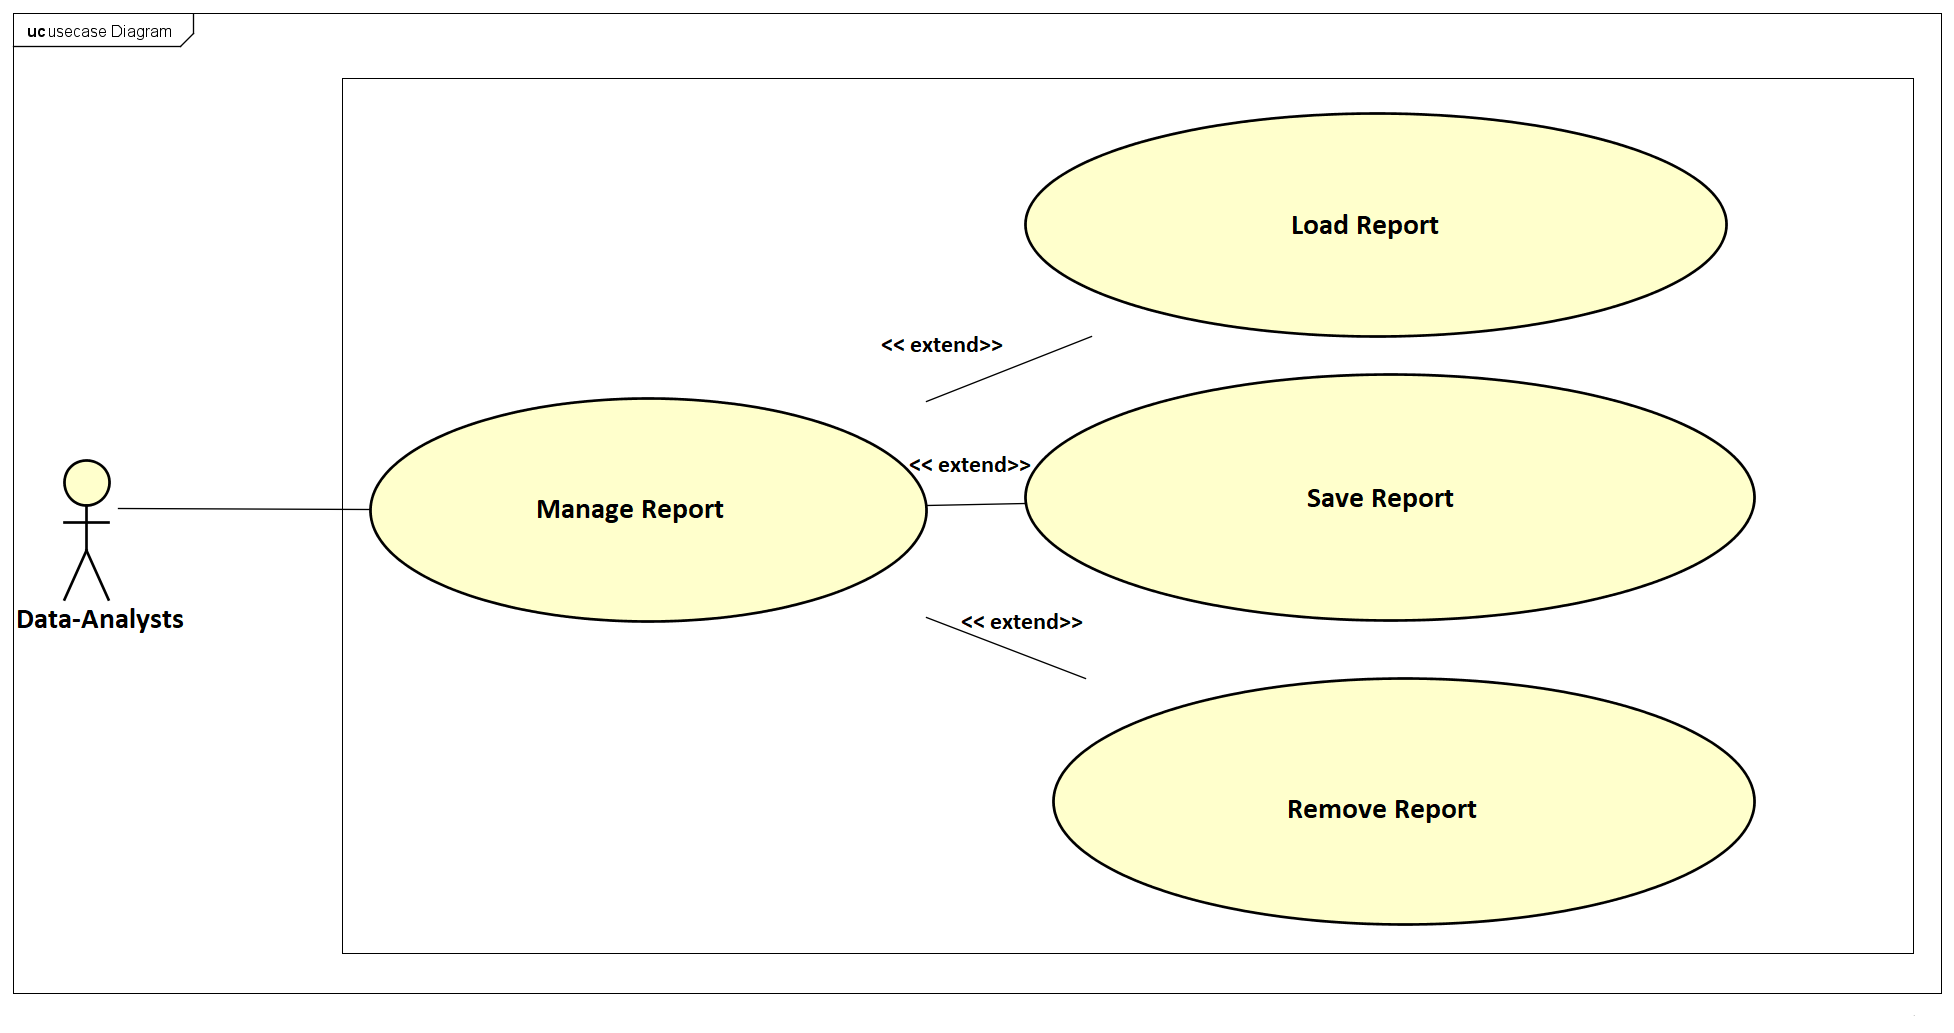
\includegraphics[width=1.0\textwidth]{manageReport.png}
	 	\caption{display reports Use Case Diagram}
	 	
	 \end{figure}
  Description of the scenario ``display reports'' in the table below.
  
   \begin{table}
  	\centering
  	\begin{tabular}{|c|p{10cm}|}
  		\hline 	
  		\textbf{Pre-Conditions } & load MassTer Insight project has been done successfully  \\ 
  		\hline                     
  		\textbf{Nominal Scenario } &
  		\begin{enumerate}
  			\item The application display by default the first optimization report.
  			\item The user gets first report through drop down.
  			\item The application display list channel related to the first optimisation report throught checkboxes list.
  			\item The application display optimisation constraints \& optimisation results. 
 
  	   	\end{enumerate} \\ 
  		\hline 
  		\textbf{Post-Conditions} & the user got optimisation Report. \\
  		\hline 
  	\end{tabular}
  \end{table}


 \clearpage
 \newpage
 
 	 \subsubsection{select report}

 Description of the scenario ``select report'' in the table below.
 
 \begin{table}
 	\centering
 	\begin{tabular}{|c|p{10cm}|}
 		\hline 	
 		\textbf{Pre-Conditions } & load MassTer Insight project contains at least one report saved\\ 
 		\hline                     
 		\textbf{Nominal Scenario } &
 		\begin{enumerate}
 			\item The application display list reports through drop down.
 			\item The user select a report trough drop down.
 			\item The user click on the button load.   
 		\end{enumerate} \\ 
 		\hline 
 		\textbf{Post-Conditions} & The application display optimization report related to the selected report \\
 		\hline 
 	\end{tabular}
 \end{table}
 \clearpage
 \newpage
  	 \subsubsection{save report}
 
 Description of the scenario ``select report'' in the table below.
 
 \begin{table}
 	\centering
 	\begin{tabular}{|c|p{10cm}|}
 		\hline 	
 		\textbf{Pre-Conditions } & \\ 
 		\hline                     
 		\textbf{Nominal Scenario } & \\ 
 		\hline 
 		\textbf{Post-Conditions} &  \\
 		\hline 
 	\end{tabular}
 \end{table}
 \clearpage
 \newpage
   	 \subsubsection{remove report}
 
 Description of the scenario ``select report'' in the table below.
 
 \begin{table}
 	\centering
 	\begin{tabular}{|c|p{10cm}|}
 		\hline 	
 		\textbf{Pre-Conditions } & \\ 
 		\hline                     
 		\textbf{Nominal Scenario } & \\ 
 		\hline 
 		\textbf{Post-Conditions} &  \\
 		\hline 
 	\end{tabular}
 \end{table}
 \clearpage
 \newpage
 
	 \subsubsection{update settings}
	 	\begin{figure}[h]
	 	\centering
	 	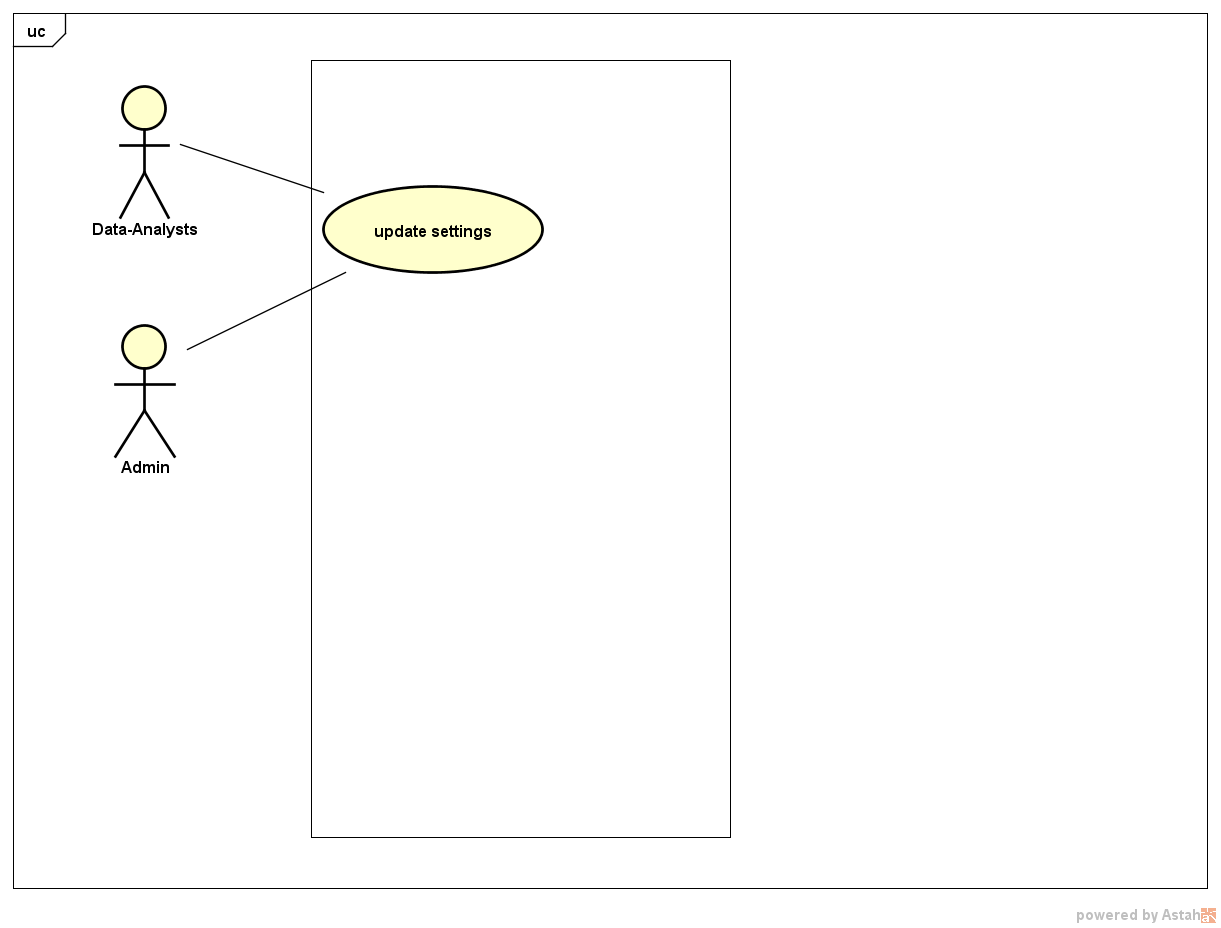
\includegraphics[width=1.0\textwidth]{updateSettings.png}
	 	\caption{update settings Use Case Diagram}
	 	
	 \end{figure}
  Description of the scenario ``update settings'' in the table below.
 \clearpage
 \newpage
	 \subsubsection{run scenario}
	 	\begin{figure}[h]
	 	\centering
	 	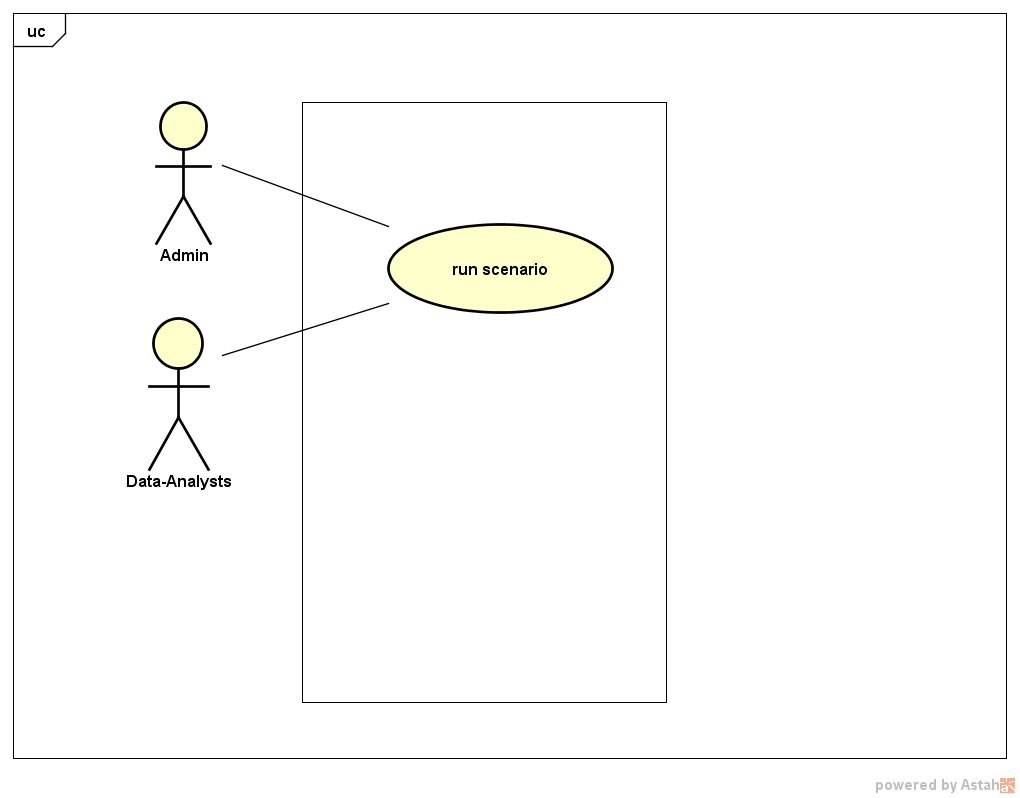
\includegraphics[width=1.0\textwidth]{runScenario.png}
	 	\caption{run scenario Use Case Diagram}
	 	
	 \end{figure}
	 Description of the scenario ``run scenario'' in the table below.
	
	\clearpage
	\newpage
	
	\section{Conclusion}
	This chapter has allowed us to identify the actors that may interact with the developed system, to define the functional and non-functional requirements of the project and modeling the use case diagrams.
	\\
	In what follows, we present the general and detailed conception phase of the System.  
	
\end{document}